\subsection{Sprint 2}

\subsubsection{Introduction}

\subsubsection{UMLs}

\begin{itemize}
    \item Task ID - 17: \href{https://tree.taiga.io/project/joseluis-teran-coffeetime/us/17?milestone=392128}{Console Diagram on Taiga (Comments Section)}
    \item Task ID - 18: \href{https://github.com/Pending-Name-21/arquitecture/pull/2}{Library UML Diagram on GitHub}
    \item Task ID - 22: \href{https://github.com/Pending-Name-21/arquitecture/pull/3}{Tic Tac Toe UML Diagram on GitHub}
\end{itemize}

\subsubsection{Spikes}

As we mentioned before, there were some Spikes to work with and here is the documentation generated by them:

\begin{itemize}    
    \item Task ID - 19: \href{https://docs.google.com/document/d/1a6wyQA0LM5thyAfOsWnkG-fTLcThvrsVPOGmFcoqkvw/edit?usp=sharing}{Graphic Libraries Documentation on Google Docs}
    \item Task ID - 20: \href{https://github.com/Pending-Name-21/console/tree/vm-spikes/jni_spike}{JNI Documentation on GitHub}
    \item Task ID - 21: \href{https://github.com/Pending-Name-21/console/blob/vm-spikes/shared-memory/README.md}{Shared Memory Documentation on GitHub}
    \item Task ID - 24: \href{https://universidadsalesian-my.sharepoint.com/:w:/g/personal/axel_ayala_9412013_usalesiana_edu_bo/EZlHobuXqW5AmffmDNnGaKYBdpordz1QlVJk88Pe_6S7HQ?e=DymfMq}{Input Listener Documentation on Word}
\end{itemize}

\subsubsection{POCs}

In this Sprint, we had no Proofs of Concept (POCs).

\subsubsection{Technical Justification}

During Sprint 2, 

\subsubsection{High - Level Architecture}

The architecture followed in this sprint was based on the initial architecture.

\begin{itemize}
    \item Architecture: \href{https://github.com/Pending-Name-21/arquitecture/pull/1/files}{Architecture Initial Version}
    You can see it on: 
    \item C4 DSL: \href{https://structurizr.com/dsl}{Visualizer}
\end{itemize}

\subsubsection{Impediments}
\href{https://docs.google.com/spreadsheets/d/1ty_hOe11I5BHMMoJYUfMxHD2sC9OoST2Nor8Q2Cqvq0/edit?usp=sharing}{impediments}

\PassOptionsToPackage{unicode}{hyperref}
\PassOptionsToPackage{hyphens}{url}
\documentclass{article}
\setcounter{secnumdepth}{3}

\usepackage{amsmath,amssymb}
\usepackage{lmodern}
\usepackage{iftex}
\usepackage[letterpaper, margin=1in, top=0.5in, bottom=1in]{geometry}
\usepackage{listings}
\usepackage{color}
\usepackage{titling}
\usepackage{graphicx}
\usepackage{hyperref}

\ifPDFTeX
  \usepackage[T1]{fontenc}
  \usepackage[utf8]{inputenc}
  \usepackage{textcomp} 
\else 
  \usepackage{unicode-math}
  \defaultfontfeatures{Scale=MatchLowercase}
  \defaultfontfeatures[\rmfamily]{Ligatures=TeX,Scale=1}
\fi
\IfFileExists{upquote.sty}{\usepackage{upquote}}{}
\IfFileExists{microtype.sty}{
  \usepackage[]{microtype}
  \UseMicrotypeSet[protrusion]{basicmath} 
}{}
\makeatletter
\@ifundefined{KOMAClassName}{
  \IfFileExists{parskip.sty}{
    \usepackage{parskip}
  }{
    \setlength{\parindent}{0pt}
    \setlength{\parskip}{6pt plus 2pt 2pt}}
}{
  \KOMAoptions{parskip=half}}
\makeatother
\usepackage{xcolor}
\usepackage{graphicx}

\makeatletter
\def\maxwidth{\ifdim\Gin@nat@width>\linewidth\linewidth\else\Gin@nat@width\fi}
\def\maxheight{\ifdim\Gin@nat@height>\textheight\textheight\else\Gin@nat@height\fi}
\makeatother
\setkeys{Gin}{width=\maxwidth,height=\maxheight,keepaspectratio}
\makeatletter
\def\fps@figure{htbp}
\makeatother
\setlength{\emergencystretch}{3em} 
\providecommand{\tightlist}{
  \setlength{\itemsep}{0pt}\setlength{\parskip}{0pt}}

\ifLuaTeX
  \usepackage{selnolig}  
\fi
\IfFileExists{bookmark.sty}{\usepackage{bookmark}}{\usepackage{hyperref}}
\IfFileExists{xurl.sty}{\usepackage{xurl}}{} 
\urlstyle{same}
\hypersetup{
  hidelinks,
  pdfcreator={LaTeX via pandoc}}

\title{Artifacts - Sprint 2}
\date{}

\begin{document}

\maketitle

\hypertarget{burndownchart-s2}{
\section{Burn Down Chart}\label{Burn Down Chart S2}}
\href{https://tree.taiga.io/project/joseluis-teran-coffeetime/taskboard/sprint-2-12274}{Link: Sprint 2 Board on Taiga}.

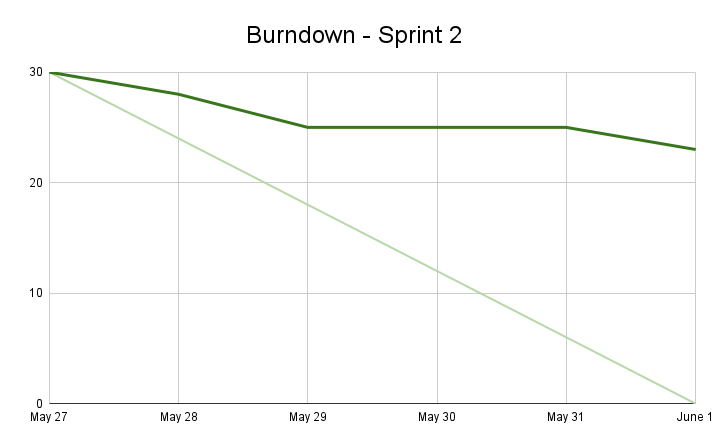
\includegraphics[width=\textwidth]{./assets/Burndown - Sprint 2.png}

\hypertarget{startstopcontinueactionitems-s2}{
\section{Start-Stop-Continue-Action Items}\label{Start-Stop-Continue-Action Items S2}}
\href{https://miro.com/app/board/uXjVKDO7l8M=/?moveToWidget=3458764590247693277&cot=14}{Link: Start-Stop-Continue-Action Items Sprint 2 on Miro}.

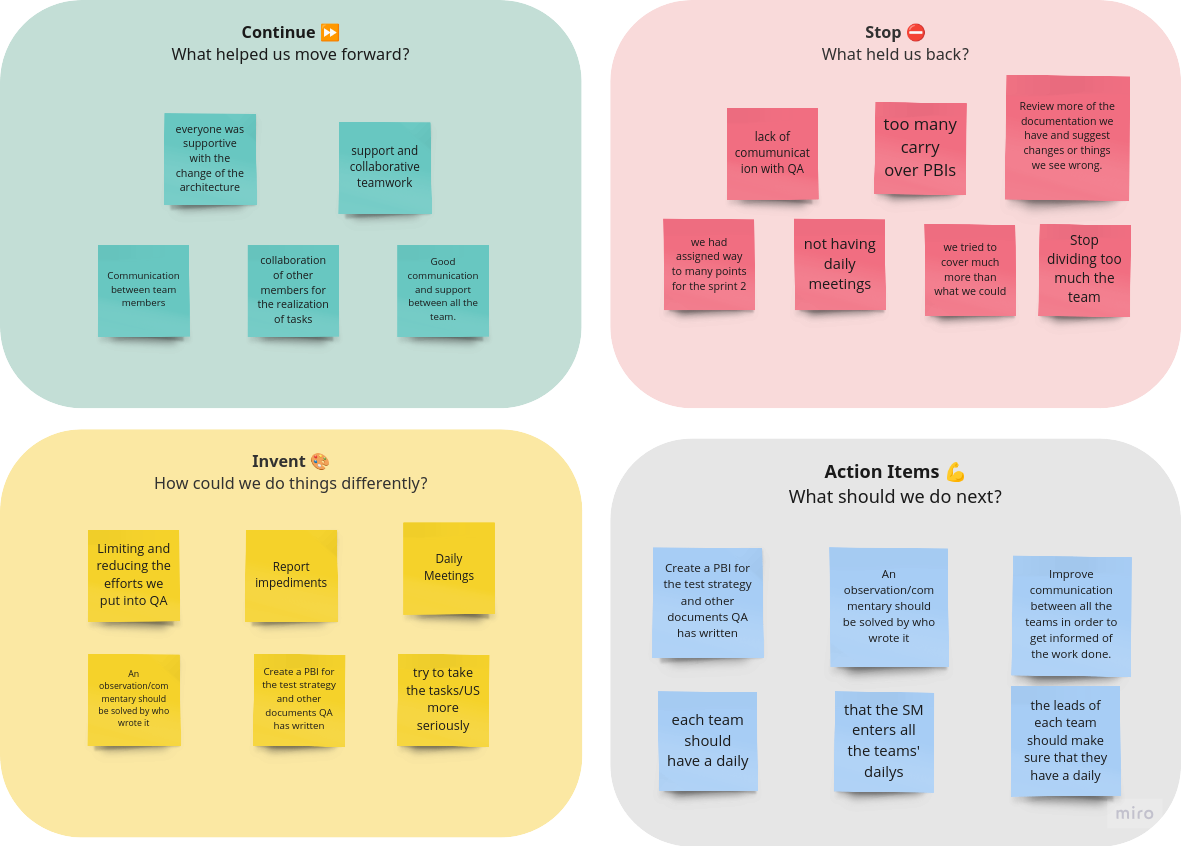
\includegraphics[width=\textwidth]{./assets/retrospective-s2.png}

\end{document}

\subsubsection{Backlog - Sprint 2}

\subsubsection*{Task Board}
\href{https://tree.taiga.io/project/joseluis-teran-coffeetime/taskboard/sprint-2-12274}{Sprint 2 Task Board}

\subsubsection*{Completed User Stories}

\begin{enumerate}
    \item \textbf{71 Pacman Mockups and Sprites} \\
    \textit{Assigned to:} Sebastian Barra \\
    \textit{Status:} Done in Sprint
    \item \textbf{18 UML: Library} \\
    \textit{Assigned to:} Santiago Concha (carryover from last sprint) \\
    \textit{Status:} Done in Sprint
    \item \textbf{19 Spike: Graphics Libraries for Console} \\
    \textit{Assigned to:} Jose Luis Teran (carryover from last sprint)\\
    \textit{Status:} Done in Sprint
    \item \textbf{20 Spike: Console with JNI} \\
    \textit{Assigned to:} Fabian Romero(carryover from last sprint)\\
    \textit{Status:} Done in Sprint
    \item \textbf{64 Input Management} \\
    \textit{Assigned to:} Luiggy Mamani and Axel Ayala \\
    \textit{Status:} Done in Sprint
    \item \textbf{91 Sound Management} \\
    \textit{Assigned to:} Alex Paca \\
    \textit{Status:} Done in Sprint
    \item \textbf{76 Input Handler for the Bridge} \\
    \textit{Assigned to:} Gabriel Concha and Fabian Romero \\
    \textit{Status:} Done in Sprint
    \item \textbf{107 Update Handler} \\
    \textit{Assigned to:} Gabriel Concha and Fabian Romero \\
    \textit{Status:} Done in Sprint
    \item \textbf{114 QA - Test Cases for Games} \\
    \textit{Assigned to:} Josue Prado and Luis Espinoza \\
    \textit{Status:} Done in Sprint
\end{enumerate}

\subsubsection*{Carryover User Stories}

\begin{enumerate}
    \item \textbf{88 Implementation of Render Handler} \\
    \textit{Assigned to:} Fabian Romero and Sebastian Sebastian Barra\\
    \textit{Status:} Carryover
    \item \textbf{72 Pacman UML} \\
    \textit{Assigned to:} Victor Villca, Jhael Arce and Ronaldo Mendoza \\
    \textit{Status:} Carryover
\end{enumerate}


